\section{Finance Ontology}\label{sec:result_f_ontology}
In this section, results from the crowdsourced ontology validation in the domain of finance are presented. A detailed discussion of the ontology used as a baseline for all calculations is done in \hyperref[sec:evaluation_datasets]{Section~\ref*{sec:evaluation_datasets}}.

As with the other datasets the method~\emph{Embedded Context} performed quite well. In fact, it outperformed all other approaches, both in terms of precision as well as recall, yielding the highest value of F-Measure. A detailed comparison of all methods for this dataset is given in~\hyperref[table:bench_p_r_f_finance]{Table~\ref*{table:bench_p_r_f_finance}}. On the other end of the table is the ontology validation without any context enrichment~(\emph{None}). This is in line with our initial hypothesis that motivated the use of concept descriptions. We also noticed the relatively high number of recall for all ontology validation approaches. The same observation was made for the other datasets as well. Indeed, crowd workers tend to decline concepts in case of uncertainty or lack of additional information.
\begingroup
\renewcommand{\arraystretch}{1.5}
\begin{table}
	\begin{tabularx}{\textwidth}{l c*{3}{Y}}
		\toprule
		Method & Precision & Recall & F-Measure \\
		\midrule
		 Embedded Context & 0.797 & 0.985 & 0.881 \\
		 External Source & 0.794 & 0.944 & 0.862 \\
		 Neighbouring Nodes & 0.756 & 0.949 & 0.842 \\
		 None & 0.734 & 0.963 & 0.833 \\
		\bottomrule
	\end{tabularx}
	\caption{Aggregated results on the Finance Ontology~(ranked by F-Measure)}
	\label{table:bench_p_r_f_finance}
\end{table}
\endgroup

Another metric we used to measure the performance of ontology validation is Inter-rater agreement. 
\hyperref[fig:hist_agreement_finance_all]{Figure~\ref*{fig:hist_agreement_finance_all}} depicts the distribution of the agreement ratio among all validated concepts. For comparability, all methods were merged into one chart and grouped by the level of agreement. Again, the method~\emph{Embedded Context} performed best followed by the method~\emph{Neighbouring Nodes} as indicated by the red bar. It shows both, a high level of full agreement~($1$) and low level of little agreement~($0.6$). 
\begin{sidewaysfigure}
  	 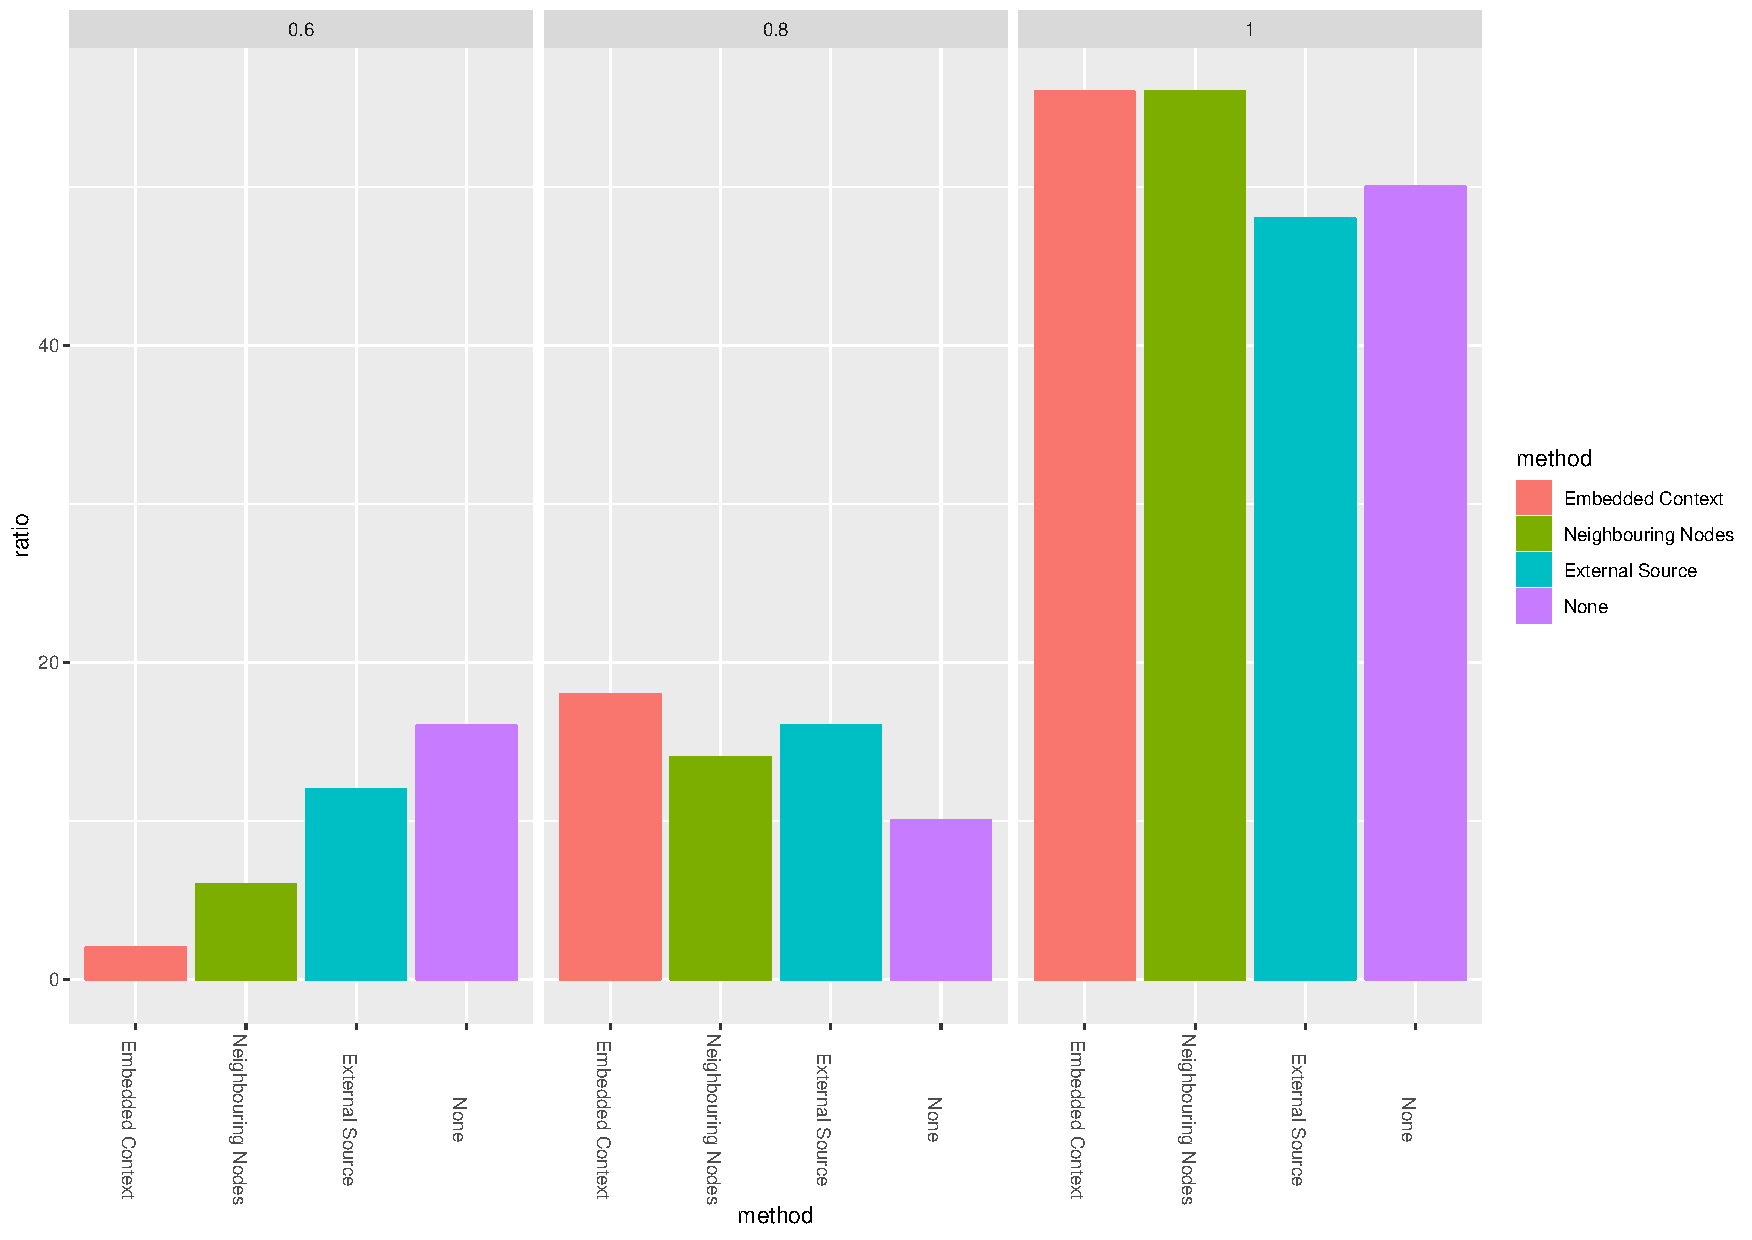
\includegraphics[width=\textwidth]{plots/finance/hist_agreement}
  	 \caption{Histogram plots of the Inter-rater Agreement}\label{fig:hist_agreement_finance_all}
\end{sidewaysfigure}


Reference to Histogram plots~\hyperref[fig:hist_level_finance_all]{Figure~\ref*{fig:hist_level_finance_all}}.
\begin{figure}
    \centering
    \begin{subfigure}[b]{0.4\textwidth}
        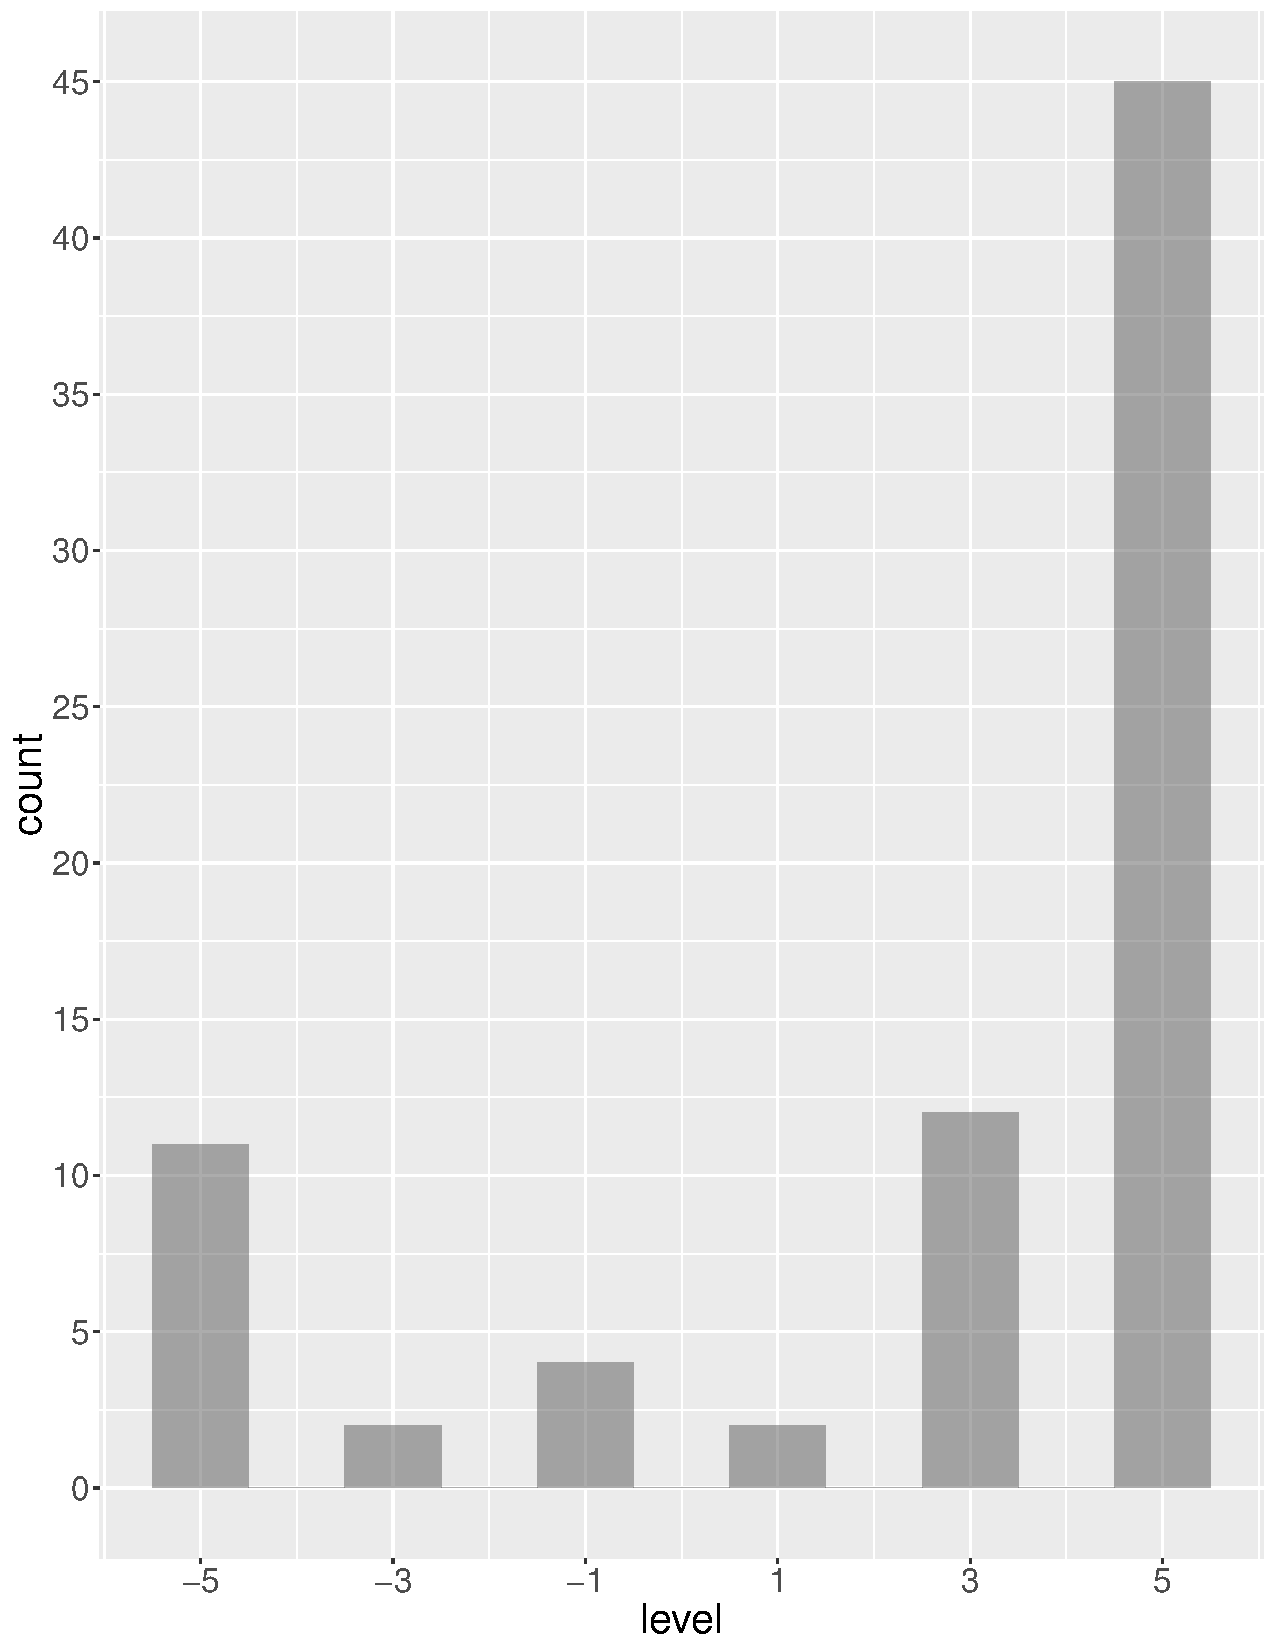
\includegraphics[width=\textwidth]{plots/finance/hist_level_nn}
        \caption{Neighbouring Nodes}
        \label{fig:hist_level_finance_nn}
    \end{subfigure}
    ~
    \begin{subfigure}[b]{0.4\textwidth}
        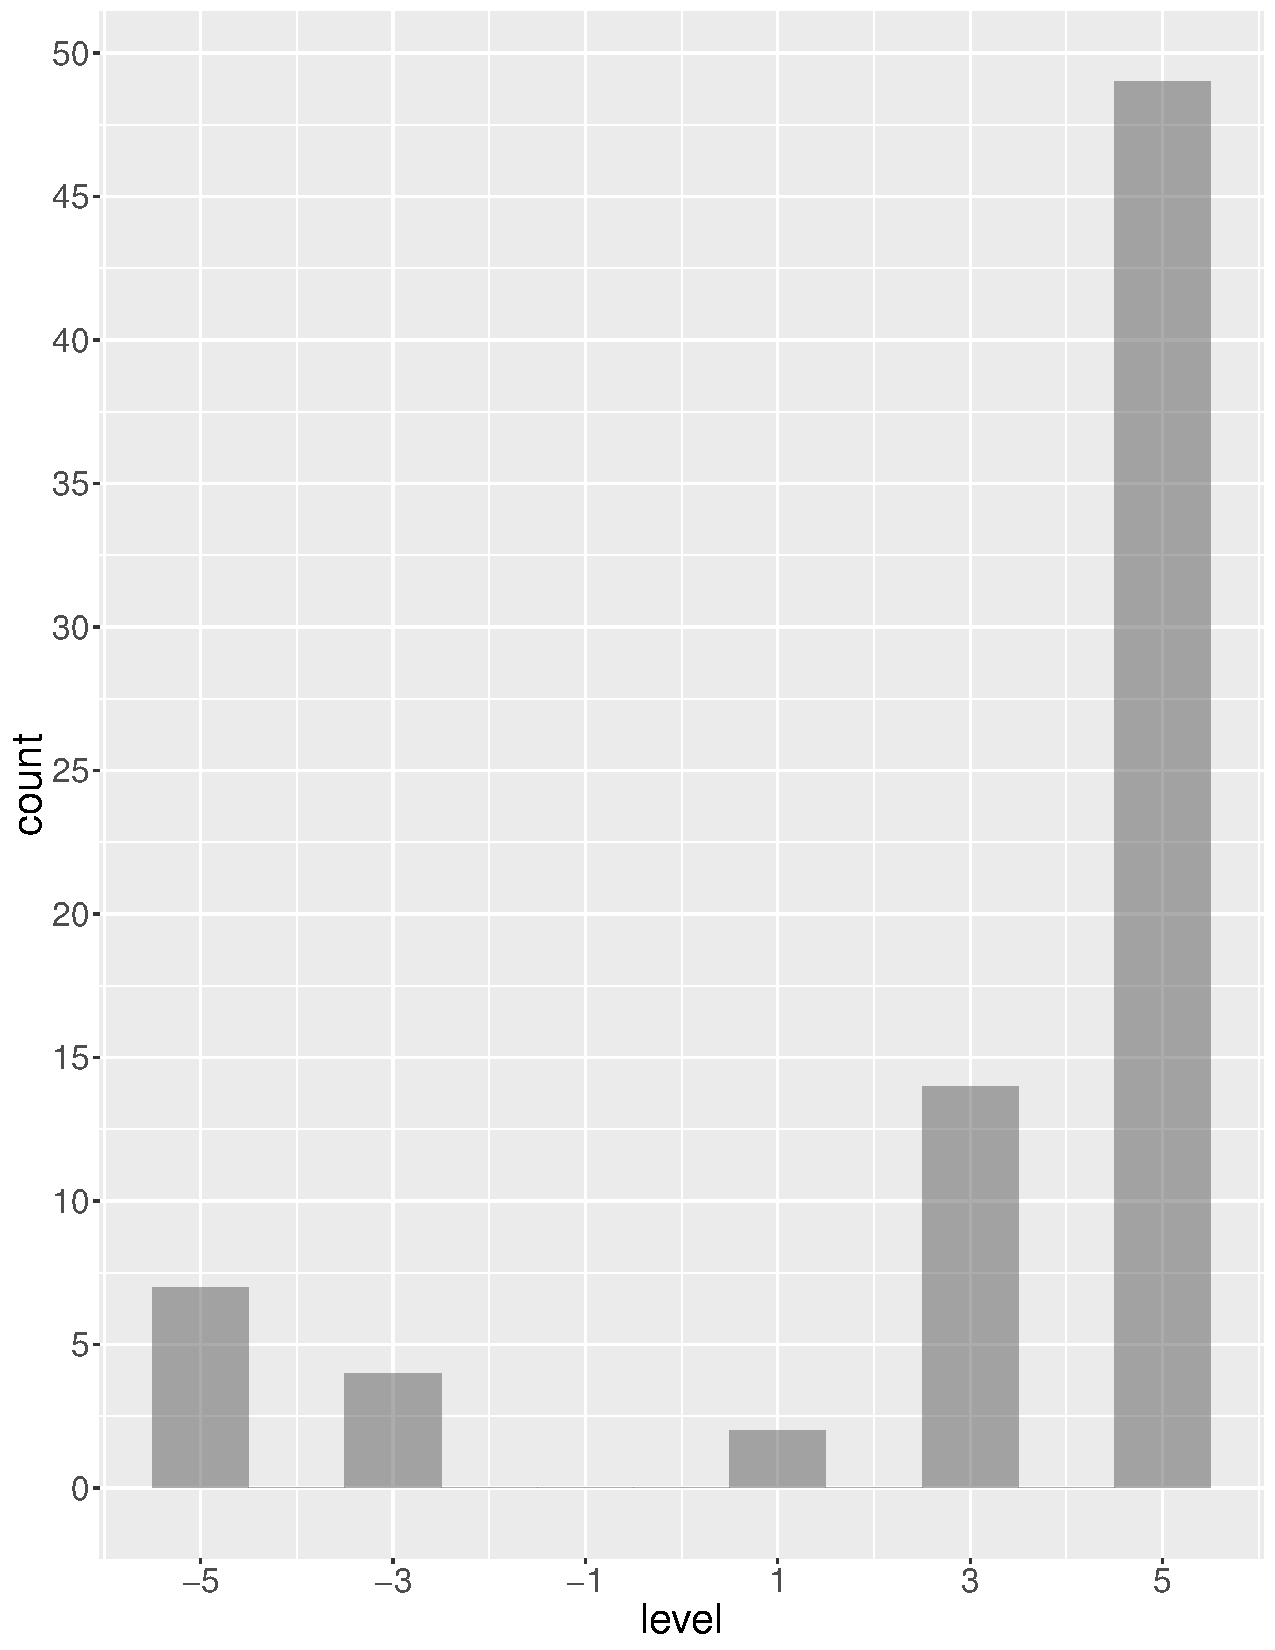
\includegraphics[width=\textwidth]{plots/finance/hist_level_ec}
        \caption{Embedded Context}
        \label{fig:hist_level_finance_ec}
    \end{subfigure}
    ~
    \begin{subfigure}[b]{0.4\textwidth}
        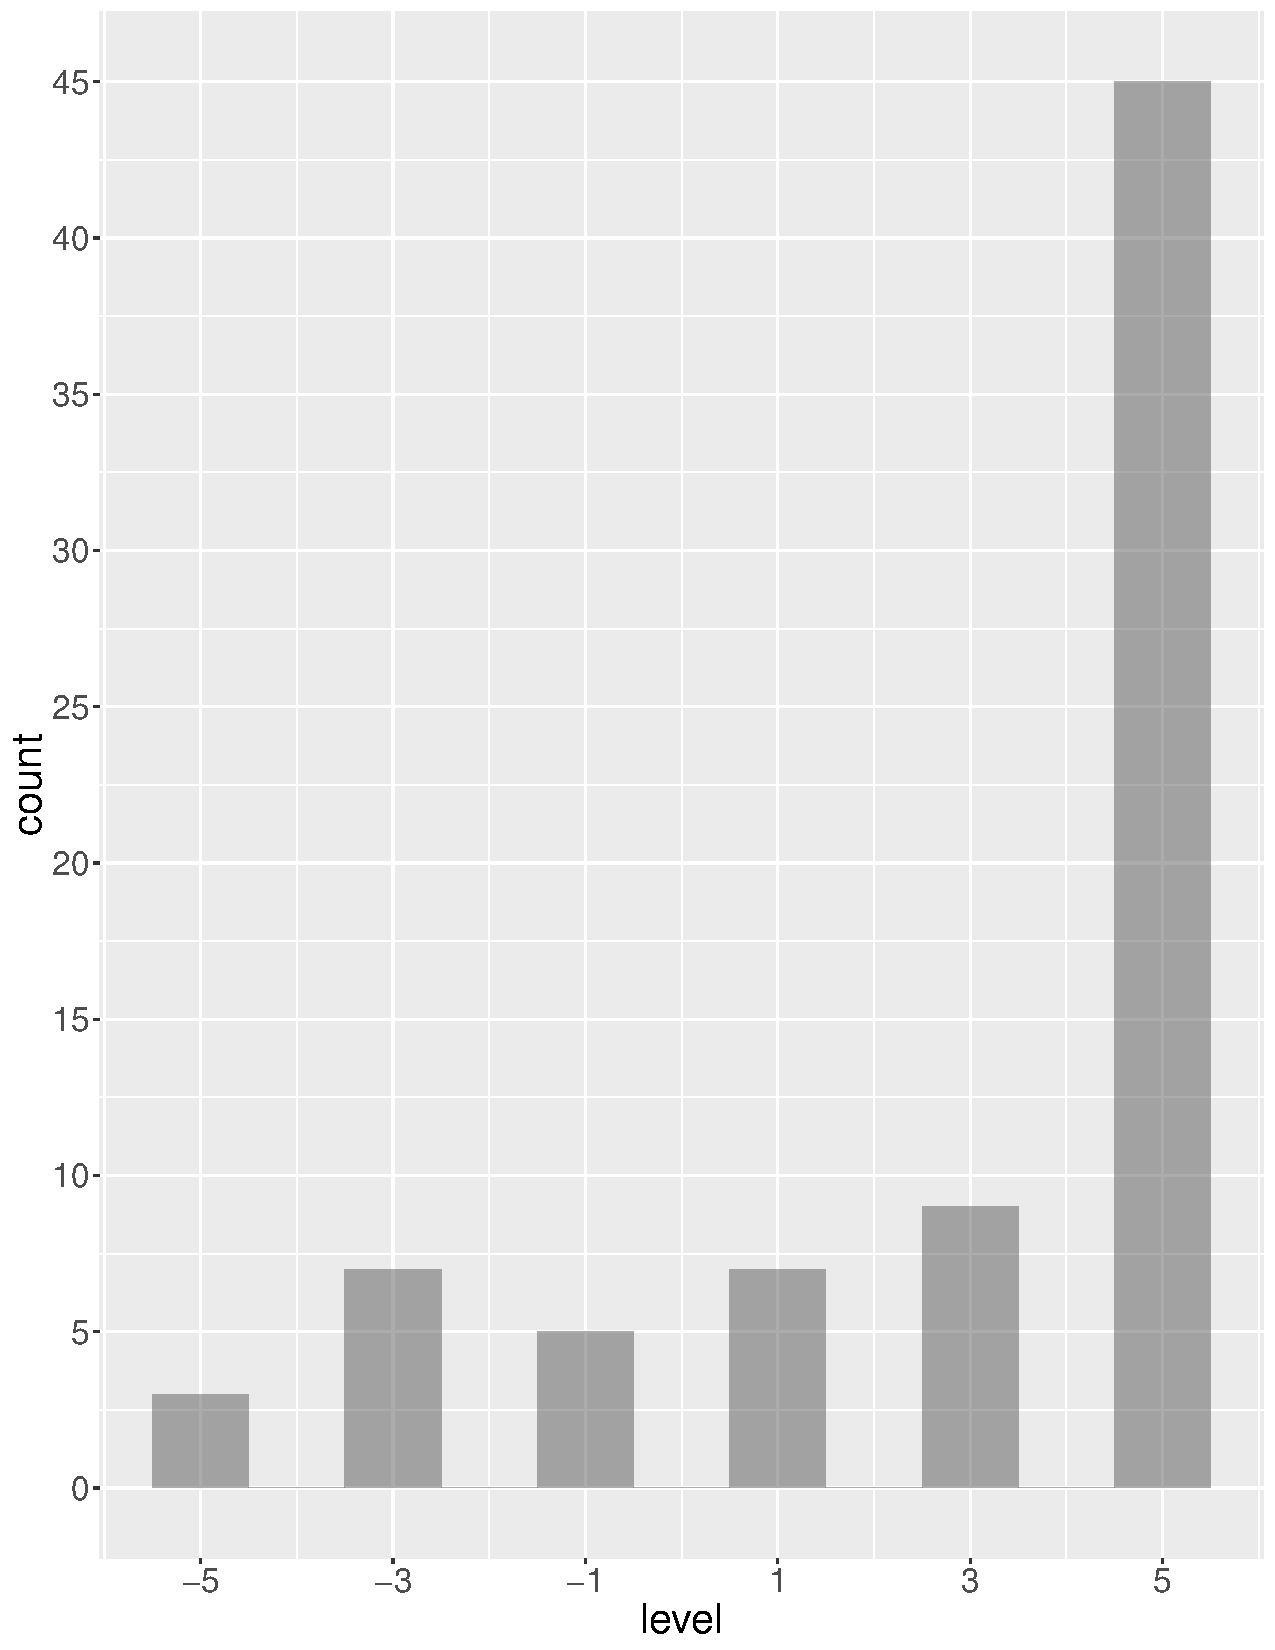
\includegraphics[width=\textwidth]{plots/finance/hist_level_es}
        \caption{External Source}
        \label{fig:hist_level_finance_es}
    \end{subfigure}
    ~
    \begin{subfigure}[b]{0.4\textwidth}
        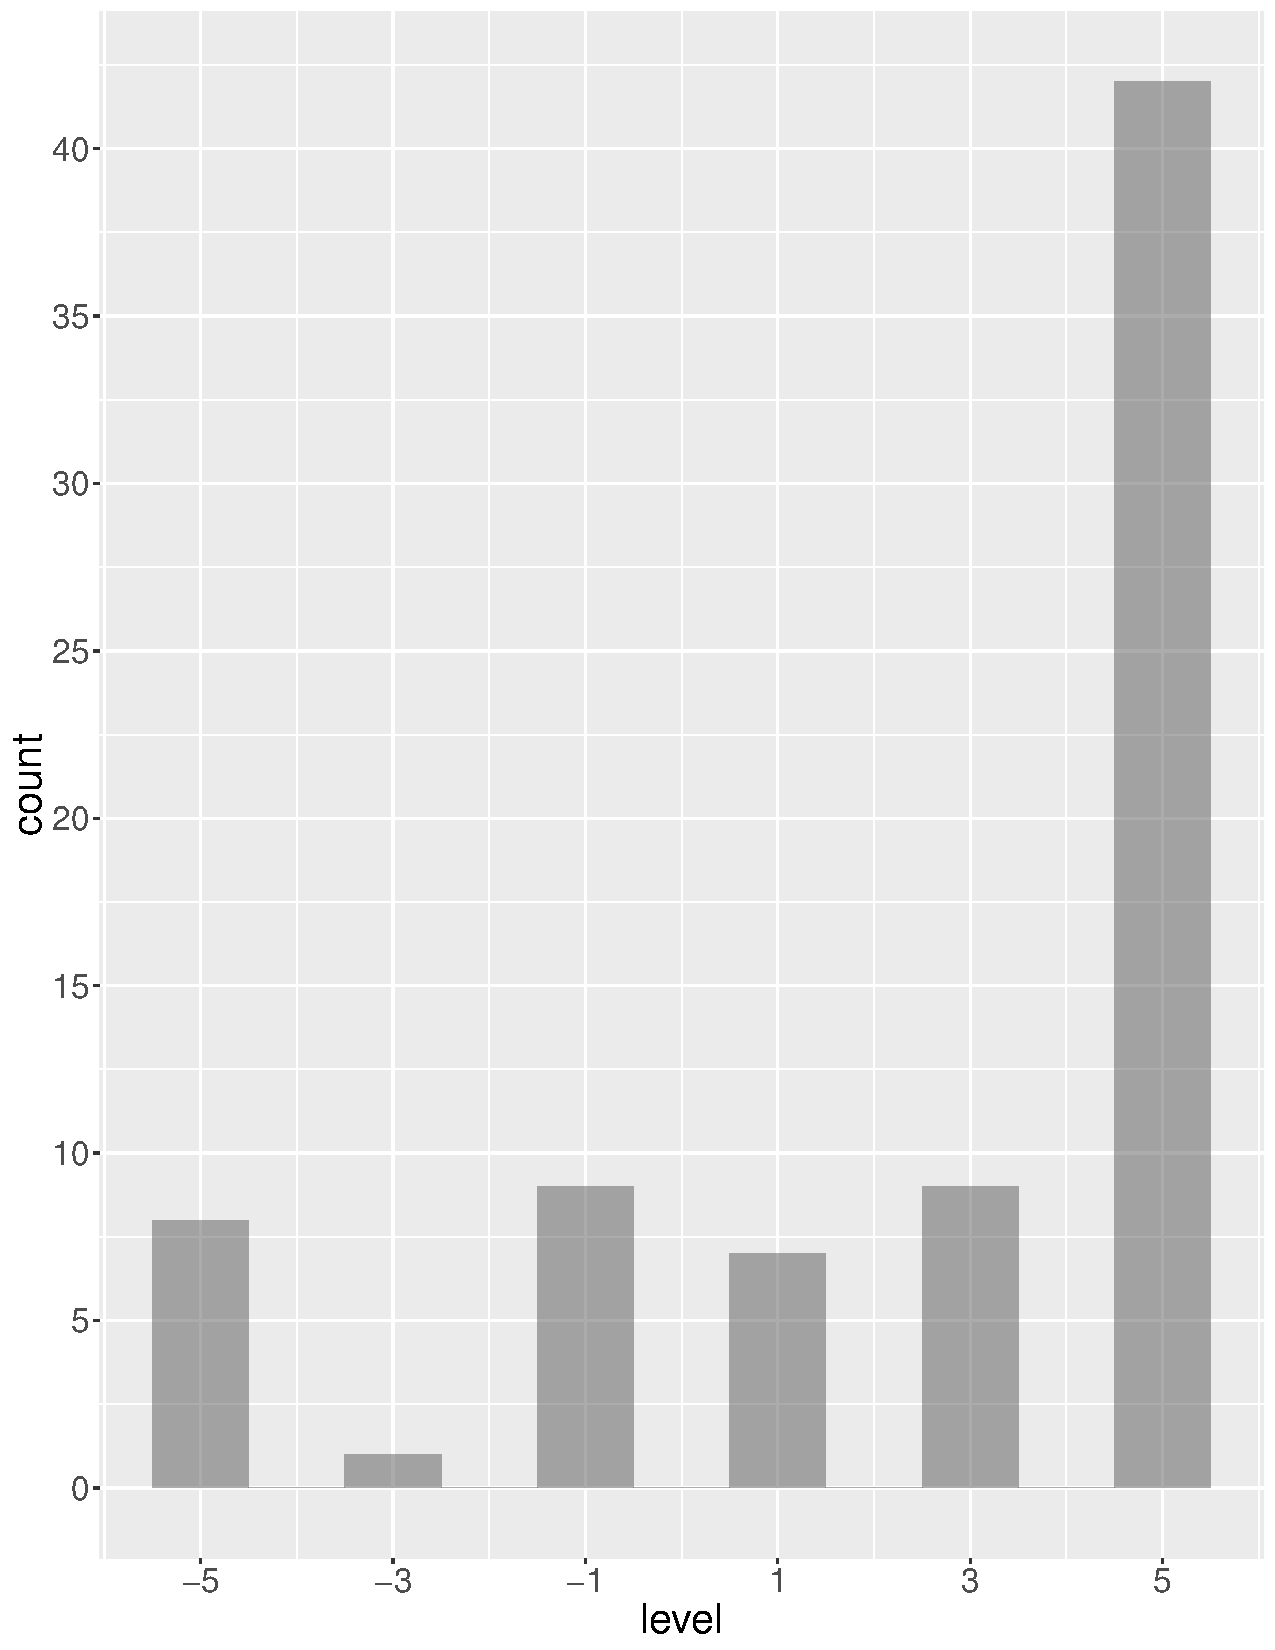
\includegraphics[width=\textwidth]{plots/finance/hist_level_none}
        \caption{None}
        \label{fig:hist_level_finance_none}
    \end{subfigure}
    \caption{Histogram plots of the correct/incorrect judgements}\label{fig:hist_level_finance_all}
\end{figure}

Reference to agreement level~~\hyperref[table:level_corr_incorr_finance]{Table~\ref*{table:level_corr_incorr_finance}}.
\begingroup
\renewcommand{\arraystretch}{1.5}
\begin{table}
	\begin{tabularx}{\textwidth}{l c*{4}{Y}}
		\toprule
		Method & mean & median & $1^{st}$ quartile & $3^{rd}$ quartile \\
		\midrule
		 Embedded Context & 3.18 & 5.00 & 3.00 & 5.00 \\
		 External Source & 2.87 & 5.00 & 1.00 & 5.00 \\
		 Neighbouring Nodes & 2.61 & 5.00 & 2.50 & 5.00 \\
		 None & 2.53 & 5.00 & 1.00 & 5.00 \\
		\bottomrule
	\end{tabularx}
	\caption{Summary statistics concerning agreement level on the Finance Ontology~(ranked by mean value)}
	\label{table:level_corr_incorr_finance}
\end{table}
\endgroup